%\documentclass[fleqn]{book}
\documentclass[11pt]{amsbook}

\usepackage[turkish]{babel}

%\usepackage{../HBSuerDemir}	% ------------------------
\usepackage{../Ceyhun}	% ------------------------
\usepackage{../amsTurkish}


\begin{document}
% ++++++++++++++++++++++++++++++++++++++
\hPage{234}
% ++++++++++++++++++++++++++++++++++++++

Düğümlerin oluşturduğu ve 5 uzunlukta bir Ç çevresi vardır. Bitişik düğümler aynı renge boyanamayacağı için bu düğümlerden en az ikisi aynı renktedir. Genellemeden birşek yitirmeksizin $d_i \ (1\leq i \leq 4)$ nin $i$ ye , $d_5$ in de 2 ye boyandığını varsayalım. (Şekil 4.5.4).

\begin{figure}[htb]
	\centering
	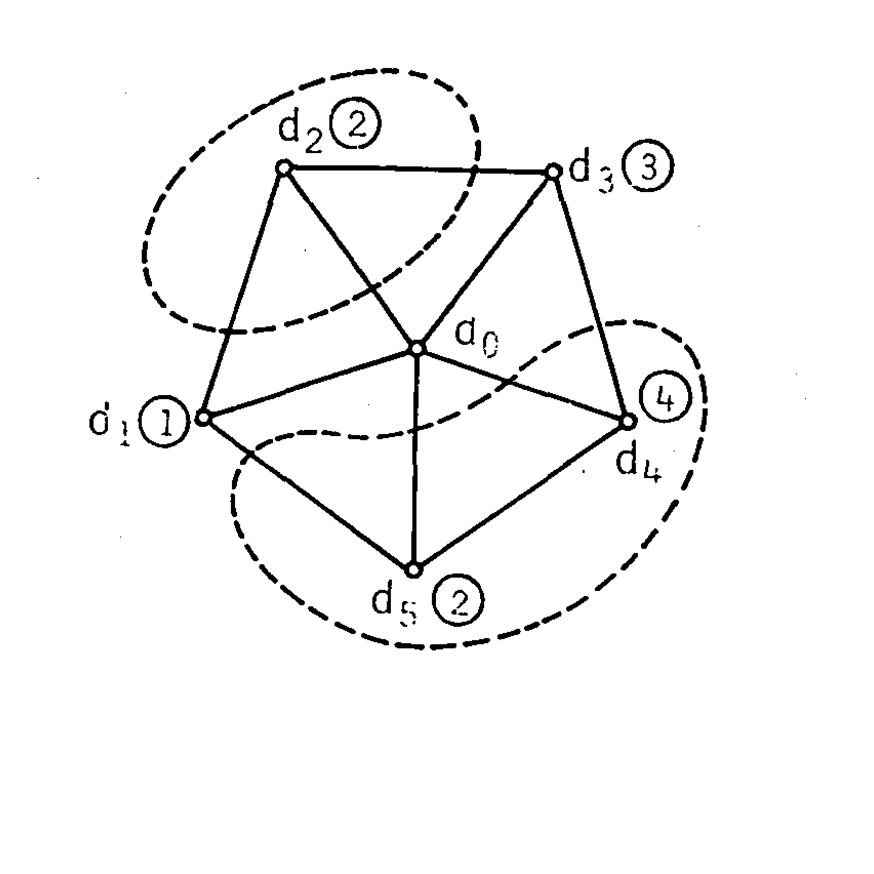
\includegraphics[width=0.45\textwidth]{images/ceyhun-234-fig01.pdf}
	\caption{Durum 2 nin incelemesi}
\end{figure}

\[ Ç_1 = Ç - (d_0)\]

olarak tanımlanan çizgeyi düşünelim. $Ç_1$ de , 1 ve 3 ile boyanmış düğümlerin irgittiği altçizge $C_2$ olsun. Eğer $d_1 $ ve $d_3$ $C_2$ nin iki ayrı parçasında ise $d_1$ in bulunduğu parçadaki düğümlerin boyanmasında 1 kullanılmamış olacaktır. Öyleyse $d_0$ ı 1 e boyayabiliriz ve $Ç(d,a)$ 4-boyanırdır.



\end{document}